\chapter{Fundamentação Teórica}
\label{chapter:fundamentacao-teorica}

\section{Considerações Iniciais}
\label{fundamentacao-teorica:inicio}

Neste capítulo é apresentado um levantamento bibliográfico sobre os principais conceitos teóricos que fundamentam este projeto. Na \autoref{fundamentacao-teorica:linguas-sinais}, o conceito de línguas de sinais é abordado, com ênfase na caracterização do tema tendo em vista o contexto educacional, bem como os principais desafios e problemas associados. A \autoref{fundamentacao-teorica:tic} relaciona os conceitos de tecnologia e educação, apresentando suas principais ferramentas de apoio ao ensino e aprendizagem, as quais têm grande potencial no suporte à educação inclusiva. Por fim, na \autoref{fundamentacao-teorica:fim} as considerações finais relacionadas aos conceitos fundamentados são apresentadas.

\section{Línguas de Sinais}
\label{fundamentacao-teorica:linguas-sinais}

Segundo \citeonline{Honora2017}, as línguas de sinais são naturais, pois surgiram espontaneamente do convívio entre as pessoas. Elas podem ser comparadas à complexidade e à expressividade das línguas faladas, já que podem transmitir qualquer conceito, concreto ou abstrato, emocional ou racional, complexo ou simples. Tratam-se de línguas organizadas e não de simples junções de gestos, o que as caracterizariam apenas como linguagens. Sendo assim, por terem regras e serem totalmente estruturadas, são denominadas línguas.

Entretanto, tal classificação precisou de algum tempo e, principalmente, pesquisa para ser aceita formalmente. Segundo \citeonline{Quadros2019}, os estudos das línguas de sinais inicialmente tiveram como função convencer os linguistas e demais agentes de políticas linguísticas/educacionais de que elas eram, de fato, línguas. Havia uma compreensão equivocada, com base no senso comum, de que as línguas de sinais seriam universais por usarem o corpo em movimentos supostamente compreendidos como gestos. Os gestos, nesse caso, eram associados à ideia de que a produção das línguas de sinais representaria formas universais e de que elas seriam facilmente entendidas por qualquer pessoa. Desse modo, haveria apenas uma única ``linguagem'' de sinais, reduzindo o status de língua para apenas uma forma de comunicação gestual compartilhável \cite{Quadros2004}. No entanto, o reconhecimento dos níveis linguísticos nas línguas de sinais permite seu enquadramento, no campo da Linguística, tanto do ponto de vista teórico, quanto aplicado \cite{Quadros2019}.

Para \citeonline{Gesser2009}, essa suposta universalidade é uma das crenças mais recorrentes quando se fala em língua de sinais. Nessa conjuntura, embora se possa traçar um histórico das origens e apontar possíveis parentescos e semelhanças no nível estrutural das línguas humanas (sejam elas faladas ou de sinais), alguns fatores favorecem a diversificação e a mudança da língua dentro de uma comunidade linguística como, por exemplo, a extensão e a descontinuidade territorial, além da diversidade cultural oriunda desses acontecimentos.

Além disso, \citeonline{Gesser2009} afirma que o que pode ser considerado universal é o impulso dos indivíduos para a comunicação e, no caso dos usuários das línguas de sinais, esse impulso é sinalizado. Sendo assim, considerar a ideia de universalidade traz implicitamente uma tendência de simplificar a riqueza linguística em questão, sugerindo que talvez para os surdos fosse mais fácil se todos usassem uma língua única/uniforme. Nesse sentido, tendo em vista que as línguas de sinais são línguas naturais, seria improvável obter tal uniformidade, pois cada uma possui influências culturais, sociais e linguísticas particulares. %De forma complementar, essa ideia tende a ser mais plausível em línguas artificiais, mas essas não se encaixam ao contexto proposto neste trabalho.
%Mesmo que, do ponto de vista prático, tal uniformidade fosse desejável, seria improvável a existência de uma língua que, além de única, permanecesse imutável em cinco continentes.

De acordo com \citeonline{Honora2017}, as línguas de sinais distinguem-se das línguas faladas porque se utilizam do meio visual-espacial em detrimento do oral-auditivo, ou seja, na elaboração das línguas de sinais é necessário olhar os movimentos que o emissor realiza para entender sua mensagem. Já na língua falada é preciso apenas ouvi-la, sem necessariamente estar olhando para o emissor. Um exemplo é um casal de ouvintes que conversa mesmo quando estão em cômodos separados em uma casa. Por outro lado, nas línguas de sinais esta situação é impossível, pois é necessário estar ao alcance da visão para que o sinal seja notado e interpretado pelos receptores.

\citeonline{Honora2017} e \citeonline{Quadros2019} ressaltam que as línguas de sinais são vivas, pois estão em constante transformação com o surgimento de novos sinais, sendo introduzidos pela comunidade surda de acordo com a sua necessidade. Conforme apresentado anteriormente, as línguas de sinais não são universais. Portanto, cada uma tem a sua própria estrutura gramatical e, assim como não se tem uma língua falada única, também não existe uma língua de sinais universal. Além disso, mesmo países com a mesma língua falada podem possuir línguas de sinais diferentes. Um exemplo é o caso de Brasil e Portugal, países que compartilham a língua portuguesa, mas têm línguas de sinais diferentes. O contrário acontece com os Estados Unidos e o Canadá, que possuem a mesma língua falada e de sinais.

\citeonline{Quadros2019} descreve que estudos das diferentes línguas de sinais do mundo evidenciaram as especificidades dos sinais de cada país, identificando inclusive sua autonomia diante das línguas nacionalmente faladas. Essa autonomia é evidenciada também pelo fato de as línguas de sinais pertencerem a diferentes famílias linguísticas, de origens distintas das línguas faladas em seus respectivos países. Por exemplo, a Libras tem origem na LSF (Língua de Sinais Francesa), enquanto a LGP (Língua Gestual Portuguesa) tem origem na STS (Língua de Sinais Sueca). Considerando essas origens, apesar de a língua falada ser a portuguesa no Brasil e em Portugal (exceto pelas variações já estabelecidas), a Libras e a LGP são completamente diferentes, pois cada uma apresenta um conjunto de fonemas próprios, que tornam as palavras muito distintas, para não falar das diversas estruturas existentes em uma língua e noutra.

Até então, esta seção apresentou algumas das principais características das línguas de sinais: (i) são línguas e não linguagens, pois possuem uma estrutura e regras próprias; (ii) não são universais, porque surgiram naturalmente, diante das necessidades de comunicação entre grupos geograficamente e culturalmente distintos; (iii) uniformidade na língua falada não garante o mesmo com relação às línguas de sinais, a exemplo de Brasil e Portugal.

Em tempo, vale ressaltar que as temáticas apresentadas possuem uma série de terminologias que advém de diferentes áreas do conhecimento, fato que muitas vezes pode dar margem para interpretações equivocadas. Nessa perspectiva, \citeonline{Quadros2019} apresenta um glossário com um conjunto de definições especificamente selecionadas para o esclarecimento de conceitos relevantes no domínio das línguas de sinais. O glossário em questão foi adaptado, com ênfase em termos pertinentes a esta pesquisa, os quais são apresentados em formato de Tabelas no decorrer desta seção. Nesse sentido, as Tabelas \ref{tab:glossario:tipos-linguas}, \ref{tab:glossario:modalidades-linguas}, \ref{tab:glossario:representacoes-visual-espaciais} e \ref{tab:glossario:termos-usuarios} organizam tais definições, destacando-as de acordo com sua importância.

\begin{table}[htbp]
\caption{Glossário: tipos de línguas}
\label{tab:glossario:tipos-linguas}
\begin{tabularx}{\textwidth}{l|X} \hline
\textbf{Língua de sinais} & \textbf{O termo ``língua de sinais'' se refere às línguas que usam a modalidade visual-espacial. Esse termo é usado genericamente em alusão a qualquer língua de sinais específica.} \\ \hline
Língua falada & As línguas faladas são as línguas orais-auditivas, ou seja, as línguas que utilizam os canais oral (aparelho vocal) e auditivo (aparelho auditivo) para produzir e perceber a fala. Essa forma será usada neste trabalho para se opor as línguas de sinais. O termo ``língua falada'' é preferido ao termo ``língua oral'' porque as línguas de sinais também são línguas orais, no sentido de serem produzidas ``oralmente'' em oposição à forma escrita. \\ \hline
\end{tabularx}
\caption*{Fonte: \citeonline{Quadros2019}.}
\end{table}

\begin{table}[htbp]
\caption{Glossário: modalidades de línguas}
\label{tab:glossario:modalidades-linguas}
\begin{tabularx}{\textwidth}{l|X} \hline
Oral-auditiva & A língua oral-auditiva se refere às línguas faladas. O português, por exemplo, é uma língua oral-auditiva, produzida oralmente com a intenção de ser ouvida. \\ \hline
\textbf{Visual-espacial} & \textbf{As línguas de sinais são visual-espaciais, pois são articuladas no espaço por meio do corpo (mãos, face etc) e acessadas visualmente, ou seja, pela visão. Os sinais são produzidos corporalmente e vistos uns pelos outros (não utilizam sons e não são ouvidos). De forma análoga a visual-espaciais, a nomenclatura gestual-espaciais também é aceita.} \\ \hline
\end{tabularx}
\caption*{Fonte: \citeonline{Quadros2019}.}
\end{table}

Em especial, a \autoref{tab:glossario:representacoes-visual-espaciais} define formalmente os termos ``gestos'' e ``sinais''. De forma resumida, um gesto pode representar a origem de um sinal, se tornando linguístico e evoluindo sua respectiva língua de sinais. Por outro lado, ainda existem pesquisas visando a desambiguação desses termos, as quais podem culminar na gramaticalização dos gestos nas línguas de sinais. A \autoref{tab:glossario:termos-usuarios} apresenta os principais termos atribuídos aos usuários das línguas de sinais. Nesse contexto, \citeonline{Quadros2019} afirma que o termo ``surdo'' é o mais apropriado considerando os usuários das línguas de sinais, pois não carrega consigo estereótipos médicos (``deficiente auditivo'') e/ou relacionados a impossibilidade de fala (``surdo-mudo'').

Um adendo importante, ainda considerando a \autoref{tab:glossario:termos-usuarios}, é de que existem outros termos comumente atribuídos aos usuários das línguas de sinais. Neste cenário, mas em uma perspectiva mais ampla, \citeonline{Oliveira2016} apresenta que ao longo dos anos diversos termos foram considerados apropriados para representar as pessoas com algum tipo de deficiência física. Entretanto, o termo recomendado atualmente é ``Pessoa com Deficiência'' (PcD), pois ele indica que há algum tipo de deficiência sem que isso inferiorize o indivíduo. Sendo assim, o termo ``PcD'' será utilizado neste trabalho em contextos mais genéricos, onde a terminologia ``surdo'' não seja adequada.

\begin{table}[htbp]
\caption{Glossário: representações visual-espaciais}
\label{tab:glossario:representacoes-visual-espaciais}
\begin{tabularx}{\textwidth}{l|X} \hline
\textbf{Gestos} & \textbf{A Gestos representam produções a partir do corpo para se referir a diferentes níveis de comportamento com ou sem significado. Os gestos são usados tanto nas línguas faladas quanto nas línguas de sinais. Nas línguas faladas, como os gestos são produzidos pelo corpo, são facilmente identificados como gestos. No caso das línguas de sinais, os gestos se apresentam na mesma modalidade dos sinais. Assim, nem sempre é fácil identificar os gestos e os sinais como produções que apresentem fronteiras claras. Os gestos podem se fundir com os sinais e se tornarem linguísticos. Os gestos nas línguas faladas são identificados como extralinguísticos. No entanto, os estudos com as línguas de sinais têm apontado para a gramaticalização dos gestos nas línguas de sinais. Talvez os gestos também possam ser considerados elementos linguísticos nas línguas faladas.} \\ \hline
\textbf{Sinais} & \textbf{As pessoas que usam uma língua de sinais normalmente se referem às palavras que a compõem como ``sinais''. Nesse caso, os ``sinais'' correspondem às ``palavras'' de sua língua falada.} \\ \hline
\end{tabularx}
\caption*{Fonte: \citeonline{Quadros2019}.}
\end{table}

\begin{table}[htbp]
\caption{Glossário: termos comuns atribuídos a usuários de línguas de sinais}
\label{tab:glossario:termos-usuarios}
\begin{tabularx}{\textwidth}{l|X} \hline
Deficiente auditivo & Deficiente auditivo é um termo para se referir aos surdos a partir da perspectiva médica. Os surdos que integram comunidades surdas e usam uma língua de sinais normalmente não utilizam o termo deficiente auditivo, pois preferem ser chamados de surdos. Por outro lado, a expressão deficiente auditivo é utilizada por surdos que não aprendem a língua de sinais. São surdos submetidos à oralização com exclusão da língua de sinais. \\ \hline
\textbf{Surdo} & \textbf{É como se identifica a pessoa que é surda, identificação considerada a mais apropriada entre os surdos que usam a língua de sinais.} \\ \hline
Surdo-mudo & É uma forma antiga de se referir aos surdos. Atualmente, os surdos consideram essa forma politicamente incorreta, pois a expressão ``mudo'' indica impossibilidade de falar, o que não expressa, de fato, a identidade surda. Os surdos podem falar e usam uma língua de sinais para se expressarem. \\ \hline
\end{tabularx}
\caption*{Fonte: \citeonline{Quadros2019}.}
\end{table}

Com isso, temas relacionados ao domínio em questão podem ser explorados de forma adequada, tendo em vista a definição e esclarecimento das principais terminologias usadas no campo das línguas de sinais, especialmente no contexto deste trabalho. Considerando as subseções a seguir, primeiramente a Libras é apresentada em detalhes, com suas respectivas características e políticas públicas voltadas para a inclusão social. Em seguida, a educação inclusiva é abordada, com ênfase no letramento bilíngue. Por fim, alguns dos desafios e problemas identificados no contexto das línguas de sinais são discutidos.

\subsection{Libras}
\label{fundamentacao-teorica:linguas-sinais:libras}

No Brasil a história das línguas de sinais teve início em 1857, com a chegada do educador francês Hernest Huet, um ex-aluno surdo do Instituto de Paris, que trouxe consigo o conhecimento sobre o alfabeto manual francês e a LSF, tidas como as principais influências para a criação da Libras \cite{Honora2017,Almeida2015}. Por sua vez, Libras é a sigla para \textbf{Lí}ngua \textbf{Bra}sileira de \textbf{S}inais, cuja comunicação é realizada por meio de gestos, expressões faciais e corporais, características em consonância com a modalidade visual-espacial.

Nesse contexto, muitas pessoas acreditam que a Libras é um alfabeto manual, algo equivocado tendo em vista as discussões supracitadas sobre a completude linguística das línguas de sinais. De acordo com \citeonline{Gesser2009}, essa inverdade fixa-se na falácia de que as línguas de sinais são limitadas e que a única forma de expressão comunicativa seria uma adaptação das letras realizadas manualmente, convencionadas e representadas a partir da língua oral.

Segundo \citeonline{Gesser2009}, o alfabeto manual, utilizado para soletrar manualmente as palavras (também referido como datilologia), é apenas um recurso utilizado por falantes da língua de sinais. Não é uma língua, mas sim um código de representação das letras alfabéticas. Sendo assim, tem uma função relevante na interação entre os usuários da línguas de sinais, principalmente para soletrar nomes próprios (pessoas ou lugares), siglas e algum vocábulo inexistente na língua de sinais.

No Brasil, o alfabeto manual é composto de 27 sinais, contando o grafema ç que é a configuração de mão da letra c com movimento trêmulo \cite{Gesser2009}. Cada formato da mão corresponde a uma letra do alfabeto do português brasileiro (\autoref{fig:libras-alfabeto}). De forma análoga também temos os números (\autoref{fig:libras-numeros}), os quais servem de referência para uma série de outros sinais, como por exemplo os dias da semana (\autoref{fig:libras-dias-semana}).

\begin{figure}[htbp]
\caption{Libras: alfabeto manual.}
\label{fig:libras-alfabeto}
\centerline{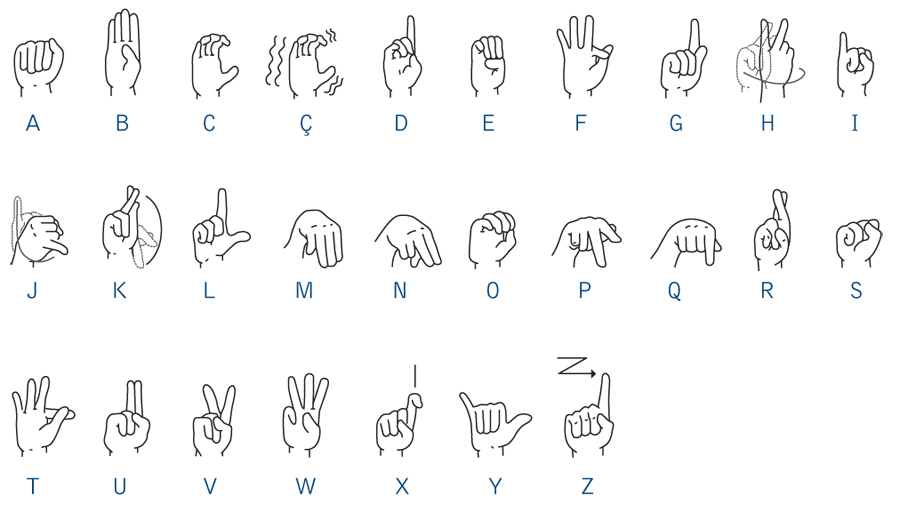
\includegraphics[width=0.95\textwidth]{images/libras-alfabeto.jpg}}
\caption*{Fonte: Centro de Educação para Surdos Rio Branco \url{www.ces.org.br}.}
\end{figure}

De modo complementar, tendo em mente a plenitude linguística da Libras, existem unidades mínimas para a formação dos sinais, tais como os fonemas nas línguas faladas. Considerando as características estruturais da Libras, seus sinais podem ser decompostos em cinco parâmetros \cite{Honora2017, Quadros2019}:

\begin{itemize}
    \item \textbf{Configuração das Mãos (CM)}: tem relação com as formas das mãos para a execução do sinal. Pode ser representado por uma letra do alfabeto, número ou outras formas de colocar a mão no momento inicial do sinal. A configuração das mãos é a representação de como estará a mão dominante (direita para os destros e esquerda para os canhotos) no momento inicial do sinal. Alguns sinais também podem ser representados pelas duas mãos;
    \item \textbf{Localização (L)}: também chamado de Ponto de Articulação (PA), diz respeito ao local onde incide a mão configurada para a execução do sinal. Pode ser alguma parte do corpo ou o sinal poderá ser realizado num espaço neutro vertical (ao lado do corpo) ou espaço neutro horizontal (na frente do corpo);
    \item \textbf{Movimento (M)}: alguns sinais têm movimento, outros não, são sinais estáticos. Movimento é o deslocamento da mão no espaço para execução do sinal;
    \item \textbf{Orientação ou Direcionalidade (O/D)}: é a direção que o sinal terá para ser executado;
    \item \textbf{Expressão Facial e/ou Corporal (EF/EC)}: muitos sinais necessitam de um complemento facial e até corporal para fazer com que sejam compreendidos. A expressão facial são as feições feitas pelo rosto para dar vida e entendimento ao sinal executado.
\end{itemize}

\begin{figure}[htbp]
\caption{Libras: números.}
\label{fig:libras-numeros}
\centerline{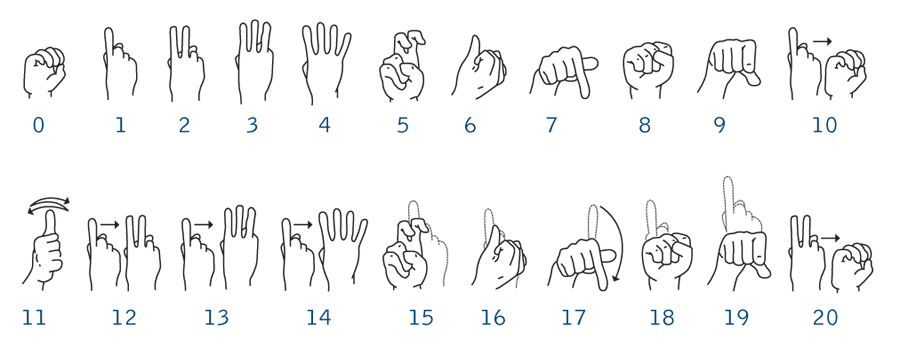
\includegraphics[width=0.95\textwidth]{images/libras-numeros.jpg}}
\caption*{Fonte: Centro de Educação para Surdos Rio Branco \url{www.ces.org.br}.}
\end{figure}

\begin{figure}[htbp]
\caption{Libras: dias da semana.}
\label{fig:libras-dias-semana}
\centerline{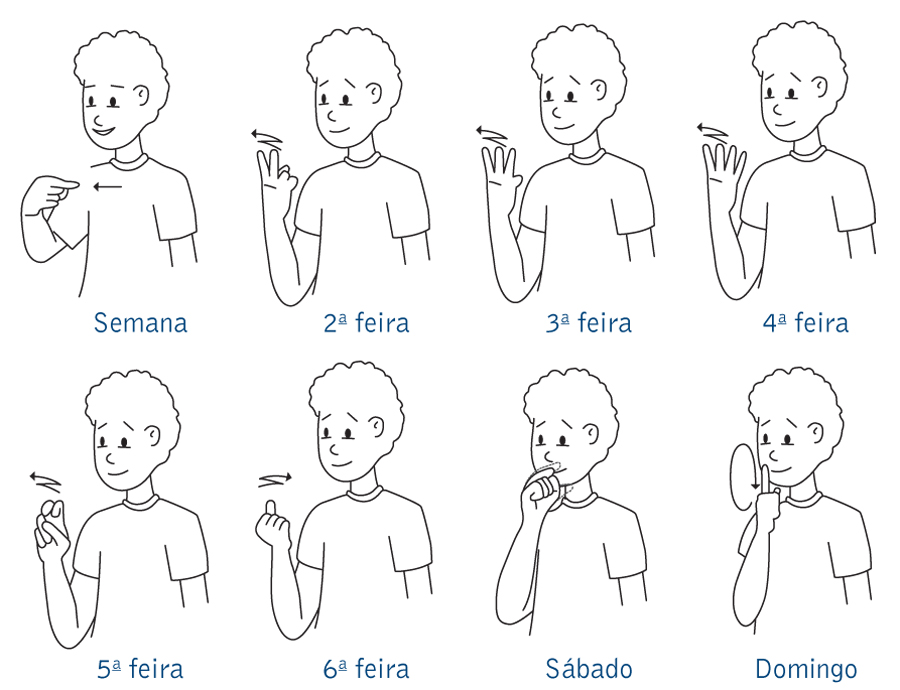
\includegraphics[width=0.8\textwidth]{images/libras-dias-semana.jpg}}
\caption*{Fonte: Centro de Educação para Surdos Rio Branco \url{www.ces.org.br}.}
\end{figure}

Considerando os parâmetros em questão, é possível ter uma dimensão da complexidade e capacidade linguística da Libras. Em particular, a \autoref{fig:libras-palavras} apresenta três palavras completamente distintas que compartilham a mesma CM (a letra ``L''). Entretanto, cada uma possui suas respectivas particularidades tendo em vista os parâmetros da Libras: (i) L: bochecha, M: semicircular para fora; (ii) L: testa, M: retilíneo repetido; e (iii) L: queixo, M: da articulação do dedo indicador -- abrir e fechar repetidamente.

\begin{figure}[htbp]
\centering
\caption{Libras: exemplos de sinais}
\label{fig:libras-palavras}
\begin{tabular}{ccc} 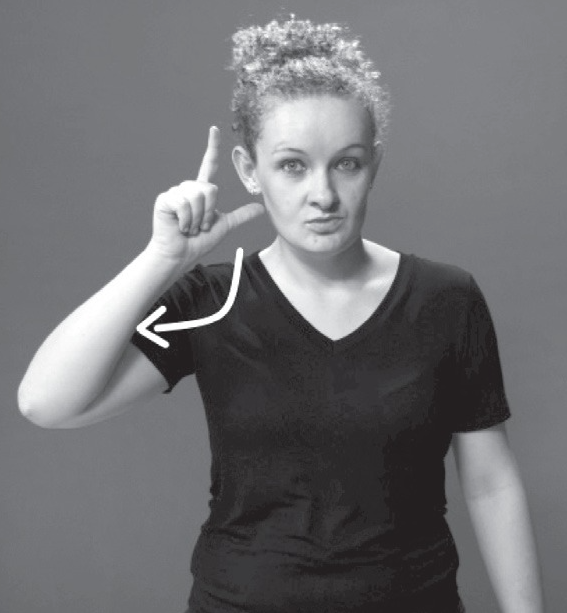
\includegraphics[width=0.331\textwidth]{images/libras-sinal-conseguir.png} &
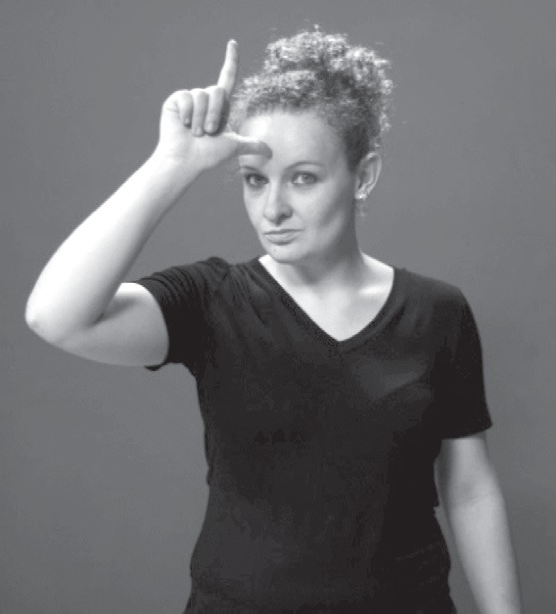
\includegraphics[width=0.325\textwidth]{images/libras-sinal-alemanha.png} & 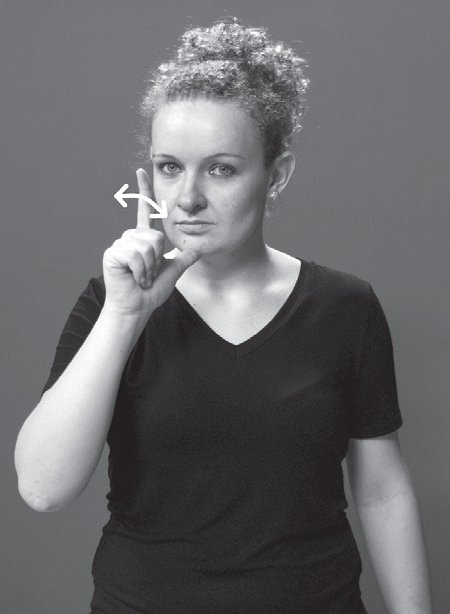
\includegraphics[width=0.264\textwidth]{images/libras-sinal-agua.png} \\
(i) Conseguir & (ii) Alemanha & (iii) Água \\
\end{tabular}
\caption*{Fonte: \citeonline{Quadros2019}}
\end{figure}

Adicionalmente, \citeonline{Quadros2019} apresenta uma visão mais técnica, na qual reitera formalmente que a Libras é uma língua dotada de todos os níveis de análise linguística. Tais características findam nossa discussão sobre a inegável integralidade da Libras enquanto língua:
\begin{itemize}
    \item Unidades mínimas (fonemas), que se combinam para formar palavras;
    \item Padrões prosódicos (realizados de forma não manual, por meio de expressões corporais ou faciais, por exemplo);
    \item Suas palavras se combinam para formar enunciados;
    \item Os enunciados apresentam proposições que podem ser analisadas do ponto de vista semântico, pragmático;
    \item Seus usos apresentam questões de ordem sociolinguística.
\end{itemize}

Sob outra perspectiva, levando em consideração o contexto social, as comunidades surdas brasileiras são representadas pela Federação Nacional de Educação e Integração de Surdos (FENEIS), que congrega várias instituições do país \cite{Quadros2019}. Uma das agendas da FENEIS era o reconhecimento legal da Libras, que culminou com a Lei nº 10.436/2002. Com isso, a Libras foi sancionada como língua de sinais oficial em 24 de Abril de 2002 \cite{Honora2017,Quadros2019,Cristiano2020}.

Segundo \citeonline{Quadros2019}, essa agenda fazia parte de um compromisso internacional estabelecido pela WFD, que inclui o reconhecimento legal das línguas de sinais de cada país. A FENEIS sempre esteve representada nas discussões em torno de questões relativas aos surdos, em especial, às políticas linguísticas voltadas para a Libras nos espaços governamentais.

Desde então, uma série de outras leis que regulamentam a Libras e assuntos relacionados à surdez vem sendo propostas. Nesse sentido, a \autoref{tab:libras:timeline} apresenta uma linha do tempo com as principais leis, decretos, portarias e resoluções sobre esses temas \cite{Cristiano2020}. Iniciativas como essas favorecem a inclusão social dos surdos, além de promover a democratização da educação inclusiva, apresentada em detalhes a seguir.

\begin{table}
\caption{Linha do tempo de leis sobre Libras e/ou Surdez.}
\label{tab:libras:timeline}
\centering
\begin{minipage}[t]{0.75\linewidth}
\color{gray}
\rule{\linewidth}{1pt}
\ytl{2002}{\href{https://www.libras.com.br/lei-10436-de-2002}{Lei nº 10.436}}
\ytl{2003}{\href{https://www.libras.com.br/portaria-3284-de-2003}{Portaria nº 3.284}}
\ytl{2004}{\href{https://www.libras.com.br/lei-10845-de-2004}{Lei nº 10.845}\\
\href{https://www.libras.com.br/lei-4304-de-2004}{Lei nº 4.304}\\
\href{https://www.libras.com.br/lei-4309-de-2004}{Lei nº 4.309}\\
\href{https://www.libras.com.br/projeto-de-lei-180-de-2004}{Projeto de Lei do Senado nº 180}}
\ytl{2005}{\href{https://www.libras.com.br/decreto-5626-de-2005}{Decreto nº 5.626}\\
\href{https://www.libras.com.br/lei-prolibras}{Prolibras}}
\ytl{2008}{\href{https://www.libras.com.br/resolucao-25-de-2008}{Resolução nº 25}\\
\href{https://www.libras.com.br/lei-11796-de-2008}{Lei nº 11.796}}
\ytl{2010}{\href{https://www.libras.com.br/lei-12319-de-2010}{Lei nº 12.319}\\
\href{https://www.libras.com.br/mensagem-532-de-2010}{Mensagem nº 532}\\
\href{https://www.libras.com.br/portaria-MEC-20-2010}{Portaria Normativa MEC 20/2010 – DOU: 08.10.2010}}
\ytl{2015}{\href{https://www.libras.com.br/lei-13146-de-2015}{Lei 13.146}}
\bigskip
\rule{\linewidth}{1pt}%
\end{minipage}%
\fautor
\end{table}

\subsection{Educação Inclusiva}
\label{fundamentacao-teorica:linguas-sinais:educacao-inclusiva}

Desde a década de 1990, surgem iniciativas globais de apoio à inclusão de PcD em escolas regulares. Em especial, a Declaração de Salamanca \cite{UNESCO1994} fomentou diretrizes básicas sobre a educação de alunos com deficiência nas escolas tradicionais para combater atitudes discriminatórias, visando uma sociedade mais inclusiva.

De acordo com a Declaração de Salamanca, o princípio fundamental da educação inclusiva é de que todos os alunos possam aprender juntos, independentemente de suas dificuldades e/ou diferenças. Por outro lado, tendo em vista a grande diversidade de PcD, essa é uma tarefa extremamente complexa, a qual exige uma nova postura tanto da gestão escolar quanto dos professores na busca de novos caminhos pedagógicos \cite{David2015}.

No Brasil, a atenção dada às minorias vem crescendo progressivamente nas últimas décadas, com o intuito de reduzir a exclusão social e proporcionar maior qualidade de vida. Em 2007, com o advento da ``Convenção dos Direitos das Pessoas com Deficiência'', os países signatários assumiram compromissos formais visando a educação inclusiva \cite{David2015,Quadros2019}. Como resultado, o Decreto nº 6.949/2009 (Artigo 24 -- Educação) foi estabelecido como uma referência para a criação de novas políticas públicas nesse contexto, as quais vêm adotando medidas para que:

\begin{citacao}
(a) As PcD não sejam excluídas do sistema educacional geral sob alegação de deficiência e que as crianças com deficiência não sejam excluídas do ensino primário gratuito e compulsório ou do ensino secundário, sob alegação de deficiência;

(b) As PcD possam ter acesso ao ensino primário inclusivo, de qualidade e gratuito, e ao ensino secundário, em igualdade de condições com as demais pessoas na comunidade em que vivem;

(c) Adaptações razoáveis de acordo com as necessidades individuais sejam providenciadas;

(d) As PcD recebam o apoio necessário, no âmbito do sistema educacional geral, com vistas a facilitar sua efetiva educação;

(e) Medidas de apoio individualizadas e efetivas sejam adotadas em ambientes que maximizem o desenvolvimento acadêmico e social, de acordo com a meta de inclusão plena.
\end{citacao}

Em especial, a inclusão escolar foi formalizada no Brasil em 2008 por meio da ``Política Nacional de Educação Especial na Perspectiva Inclusiva''. Posteriormente, com a Lei Brasileira de Inclusão (LBI) em 2015, a conciliação da legislação nacional com a última ``Convenção dos Direitos das Pessoas com Deficiência'' (2011) estabeleceu legalmente as condições de implementação do sistema educacional inclusivo em todos os níveis e modalidades \cite{Alana2019}.

Por outro lado, o paradigma inclusivo, amparado pelas políticas nacionais, demonstrou a necessidade de uma profunda reestruturação do sistema educacional brasileiro. Essa reestruturação, que se propõe a atender a diversidade de seus alunos da melhor maneira possível, culminou projetos de uma escola para todos \cite{Almeida2015}. No que se refere à inclusão de pessoas com surdez, pode-se afirmar que há uma tensão explícita entre aqueles que defendem a presença dos alunos com surdez em escolas e classes tradicionais e aqueles que lutam pela educação de surdos em instituições bilíngues \cite{Almeida2015,Quadros2019}.

Segundo \citeonline{Almeida2015}, é importante esclarecer que aqueles que defendem o fim da educação especial de surdos e sua inserção nas escolas tradicionais, sem concentrá-los numa mesma turma, argumentam que insistir na educação de surdos é retroceder na inclusão e discriminar negativamente esses alunos. Entretanto, desconsideram diversas questões, tais como as linguísticas e culturais, intrínsecas à educação de surdos, e, também, a grande heterogeneidade presente em meio às pessoas com surdez.%, desde a polarização mais comum entre surdos, no sentido cultural do termo, e pessoas com deficiência auditiva e/ou ensurdecidas, até as demais diferenças sociais, físicas, etárias, étnicas e pessoais desses indivíduos.

\citeonline{Quadros2019} defende que, no caso específico dos surdos, ``inclusão'' deveria significar acesso à educação bilíngue, em que há agrupamentos de surdos, uso da língua de sinais, ensino da língua de sinais, ensino da língua portuguesa como segunda língua e a criação de um ambiente multilíngue e multicultural.

\citeonline{Quadros2019} e \citeonline{Almeida2015} concordam que os movimentos surdos clamam por inclusão em uma outra perspectiva. Nota-se que eles entendem a inclusão como garantia dos direitos de terem acesso à educação de fato, consolidada em princípios pedagógicos que estejam adequados aos surdos. Tais proposições ultrapassam as questões linguísticas, incluindo aspectos sociais, culturais, políticos e educacionais. Sendo assim, a educação bilíngue possui grande importância na concepção da educação inclusiva para surdos, pois trata a língua de sinais e a língua falada com o mesmo grau de importância no âmbito escolar. De acordo com \citeonline{Quadros2019}, os objetivos da educação bilíngue incluem os seguintes pontos:

\begin{enumerate}[label=(\alph*),noitemsep,topsep=0pt]
    \item Legitimar a experiência visual;
    \item Assegurar o desenvolvimento socio-emocional íntegro das crianças a partir da identificação com surdos adultos (encontro surdo-surdo);
    \item Criar um ambiente linguístico-social apropriado às formas particulares de processamento cognitivo e linguístico das crianças surdas;
    \item Garantir as possibilidades para que as crianças surdas construam uma teoria de mundo;
    \item Oportunizar o acesso à informação curricular e cultural.
\end{enumerate}

Nesse contexto, \citeonline{Quadros2019} discorre que sobre duas abordagens relevantes no âmbito da educação bilíngue com Libras, as quais, idealmente, devem coexistir em uma sala de aula inclusiva. Dessa forma, surdos e ouvintes interagem naturalmente, tendo em vista as suas respectivas línguas principal (L1) e secundária (L2):

\begin{itemize}
    \item \textbf{Ensino de Libras como L1}: primeiramente, a carga horária para o ensino de Libras deve ser equivalente à carga horária da segunda língua (Português). Isso já integra a reestruturação da arquitetura escolar, pois as línguas passam a ocupar parte da carga horária de ensino de forma mais equivalente. Com isso, o aluno surdo será educado com ênfase na Libras, língua com a qual pode não ter tido contato prévio, geralmente porque ela não é a língua de convívio da maioria de seus familiares, o que caracteriza um desafio pedagógico adicional;
    \item \textbf{Ensino de Libras como L2}: para alunos ouvintes, familiares e demais pessoas envolvidas na comunidade escolar é um dos pilares da educação bilíngue, especialmente nas escolas inclusivas. Considerando um currículo no qual a Libras e a língua portuguesa compartilhem uma carga horária equivalente, os alunos ouvintes contarão com o ensino da Libras como segunda língua. A equivalência entre Libras e Língua portuguesa na distribuição da carga horária escolar é muito importante, pois legitima as duas línguas no espaço escolar ao lhes dar o mesmo status.
\end{itemize}

Por fim, \citeonline{Quadros2019} sintetiza o histórico das políticas públicas para a educação bilíngue em uma sequência de acontecimentos fundamentais, muitos dos quais foram citados previamente. Para a autora, os seguintes eventos merecem destaque: (i) Lei ``da Libras'' nº 10.436/2002; (ii) Decreto nº 5.626/2005, (iii) Convenção dos Direitos das Pessoas com Deficiência (2007, 2011); (iv) Lei nº 13.005/2014 (que estabelece o Plano Nacional de Educação para o período de 2014-2024).

%Em 2018, após dez anos da Política, segundo o Censo Escolar, o número de matrículas da educação especial (na política de educação inclusiva do Brasil) chegou a 1,2 milhão, um aumento de 70\% desde 2008. Dentre as quais, o percentual de alunos incluídos em salas regulares, que em 2008 era de 54\%, passou para 92\% em 2018 \cite{Alana2019}.

A educação inclusiva representa um avanço no modo de conceber a escolarização de PcD, indicando os suportes educacionais necessários para operacionalizá-la. Em especial, no contexto dos surdos, a educação bilíngue surge como uma forma de inclusão da Libras como uma alternativa e não uma exceção. Entretanto, ainda existem muitos desafios e problemas para uma hipotética democratização das línguas de sinais, os quais são discutidos a seguir.

\subsection{Desafios e Problemas}
\label{fundamentacao-teorica:linguas-sinais:desafios}

Nesta seção alguns dos principais desafios das línguas de sinais e educação inclusiva são apresentados. Para isso, duas vertentes de discussão são delineadas: (i) Libras é língua de herança -- regionalidades e risco de extinção das línguas de sinais nacionais e locais; (ii) Educação inclusiva para todos -- alternativas para potencialização do ensino bilíngue em âmbito nacional. 

\citeonline{Quadros2019} discute as relações de pertencimento às comunidades surdas brasileiras e associa o termo ``língua de herança'' à Libras. Segundo \citeonline{Quadros2017}, a Libras é passada de geração em geração entre surdos de uma mesma comunidade (não necessariamente dentro do núcleo familiar). Além disso, é uma língua usada, principalmente, em grandes centros urbanos de um país que possui outra língua oficial, o Português, veiculado nos meios de comunicação, documentos oficiais, órgãos públicos etc. Sendo assim, a Libras é certamente uma língua de herança.

Nesse contexto, \citeonline{Quadros2019} expande essa discussão ao classificar as línguas de sinais em: nacionais e locais. Segundo a autora, as línguas de sinais locais são usadas por surdos geralmente de pequenas comunidades situadas em espaços geográficos específicos dentro de um mesmo país. Por outro lado, nacionais são as línguas usadas por várias comunidades surdas de um país, apresentando abrangência nacional. 

A Libras, por ser difundida em todo o território brasileiro, é considerada a língua de sinais nacional. Já as línguas de sinais locais, variam entre desligadas (isoladas), rurais e de vilas (incluindo as línguas de sinais indígenas, também locais e isoladas) \cite{Quadros2017,Quadros2019}. Nesse sentido, a autora discorre sobre uma maior possibilidade de extinção das línguas de sinais locais, principalmente devido a maior disseminação da Libras que, com o tempo, poderia se consolidar por meio das novas gerações e interromper a ``tradição'' das línguas locais.

A extinção de uma língua de sinais traz consigo uma perda social e cultural imensuráveis. Nesse contexto, \citeonline{Quadros2019} apresenta evidências de que a própria Libras está em risco, não obstantes seu reconhecimento por meio de lei e as várias políticas públicas para sua valorização. Tal risco decorre da forma de transmissão da Libras, o fato de não ser transmitida de pai para filho -- a maioria das crianças surdas nasce em famílias de ouvintes monolíngues -- torna a língua suscetível a constantes reinvenções. As crianças surdas crescem sem uma língua estabelecida. Em alguns casos, na tentativa de se comunicarem, elaboram produções próprias que podem se tornar verdadeiras línguas emergentes. No entanto, muitas vezes, terão contato tardio com uma língua de sinais já estabelecida, como a Libras.

De forma complementar, \citeonline{Quadros2019} alerta que existem políticas educacionais que inviabilizam a aquisição de linguagem por meio da Libras, quando não proporcionam o desenvolvimento da criança surda com seus pares (outras crianças surdas) e com referências de adultos surdos sinalizantes da Libras. Com isso, a criança surda só virá a ter contato com a Libras tardiamente, já com vários comprometimentos de ordem linguística e cognitiva. No período sem acesso à Libras, algumas crianças têm contato superficial com professores que sabem alguns sinais e, se tiverem sorte, com intérpretes de Libras. Nesse contexto, as crianças aprendem uma sinalização que não é propriamente uma língua, estabelecida a partir de modelos que apenas incorporam algo da Libras.

Portanto, é possível concluir que a Libras também está em risco, pois as crianças vão se tornar os adultos surdos de amanhã, e os adultos surdos sinalizantes da Libras irão morrer algum dia. O legado da Libras só será mantido se as crianças surdas tiverem contato com adultos surdos sinalizantes em Libras, pois a herança linguística é transmitida pela comunidade surda, não pelas famílias \cite{Quadros2019}.

Por outro lado, ao pensar na educação inclusiva, um dos grandes desafios que se apresentam é o atendimento a todos os indivíduo, de forma igualitária, no que se refere aos direitos à educação, e que valorize a diversidade como elemento que possibilite, a todo e qualquer indivíduo, com ou sem deficiências, as ferramentas necessárias para o seu aprendizado \cite{Almeida2015}.

\citeonline{Almeida2015} afirma que os modelos de escolarização impostos aos surdos, na maioria das vezes, os desconsideraram em sua especificidade. Adicionalmente, o autor critica a atual aplicação de propostas inclusivas, ditas bilíngues, que ``mantêm de forma velada a ideia de que o surdo precisa ser reabilitado e de que a Libras é apenas mais um recurso de acessibilidade''. Essa critica é extremamente pertinente e traz a tona a diferença fundamental entre os termos acessibilidade e inclusão, no contexto dos surdos. Nesse sentido, \citeonline{Quadros2019} discorre sobre esses conceitos, com o adendo do termo exclusão (\autoref{tab:glossario:acessibilidade-exclusao-inclusao}).

\begin{table}[htbp]
\caption{Glossário: Acessibilidade, Exclusão e Inclusão}
\label{tab:glossario:acessibilidade-exclusao-inclusao}
\begin{tabularx}{\textwidth}{l|X} \hline
Acessibilidade &  Tudo o que é acessível, ou seja, tudo o que as pessoas conseguem compreender, atender, aquilo de que conseguem participar efetivamente. \textbf{No caso dos surdos, a acessibilidade começa pela língua de sinais, que os inclui na conversa, na interação, no espaço social.} Há também outros aspectos a serem considerados para garantir a acessibilidade aos surdos. Um exemplo é o espaço, que precisa ser suficientemente iluminado para ser visto pelos surdos. Locais escuros os excluem. Sinais luminosos, em vez de sinais sonoros em espaços públicos e escolas são também outro exemplo de medidas que tornam o espaço acessível ao surdo.\\ \hline
Exclusão & Exclusão envolve a privação de alguém em participar de algumas atividades ou funções. No caso dos surdos, uma das formas mais contundentes de exclusão é o uso da língua falada. \textbf{Os surdos não ouvem a língua falada, então são facilmente excluídos do que está sendo tratado.} Para evitar a exclusão dos surdos em contextos em que se usa a fala como meio de comunicação, são contratados intérpretes de línguas de sinais, tornando assim o ambiente acessível. \\ \hline
\textbf{Inclusão} & \textbf{Inclusão é um termo usado para se referir à inserção das pessoas com deficiência (em certos contextos, abrange quaisquer pessoas que apresentem marcas sociais diferenciadas, tais como negros, homossexuais, mulheres, todas consideradas relativas do ponto de vista de quem estabelece o que seria a norma) na sociedade. O termo é comumente usado para se referir à ``educação inclusiva'' (\autoref{fundamentacao-teorica:linguas-sinais:educacao-inclusiva}), na qual os surdos são incluídos, idealmente, por meio do bilinguismo.} \\ \hline
\end{tabularx}
\caption*{Fonte: \citeonline{Quadros2019}.}
\end{table}

Com base nas definições de \citeonline{Quadros2019} e as discussões preestabelecidas neste trabalho, fica evidente que os surdos almejam a inclusão, além da acessibilidade, que fica implícita em um contexto inclusivo. Isso porque o fato de um ambiente ou solução ser acessível, não garante que o mesmo seja inclusivo. Por isso, é necessário refletir sobre estratégias e ferramentas que possam auxiliar na inclusão dos surdos, em especial no âmbito educacional. Tendo isso em mente, a seção seguinte fundamenta possíveis alternativas no conjuntura das tecnologias aplicadas à educação.

\section{Tecnologia e Educação}
\label{fundamentacao-teorica:tic}

A educação e a busca por conhecimento representam, especialmente no contexto das PcD, algumas das formas mais efetivas para a inclusão social dessas pessoas. Esse cenário, associado ao rápido crescimento das Tecnologias de Informação e Comunicação (TICs), tem favorecido o surgimento de novas modalidades de ensino, proporcionando alternativas mais adequadas ao contexto dos aprendizes na atual sociedade \cite{Kukulska2005, Castrillo2014}. 

Segundo a União Internacional de Telecomunicações (ITU -- \textit{International Telecommunication Union}), agência especializada nas TICs, pela primeira vez na história mais da metade da população mundial têm acesso à Internet, o equivalente a 4 bilhões de pessoas \cite{Itu2020}. Cronologicamente, o acesso individual à rede subiu de 17\% em 2005 para 51\% em 2019, um aumento expressivo que demostra uma forte tendência para um mundo amplamente conectado. De modo adicional, o ITU apresentou uma variação dessa estimativa considerando o público jovem (15 a 24 anos). Com isso, ficou evidente que esse grupo de pessoas é muito mais ativo com relação à Internet (\autoref{fig:itu-uso-internet}).

\begin{figure}[htbp]
\caption{ITU: Porcentagem de indivíduos que usam a Internet.}
\label{fig:itu-uso-internet}
\centerline{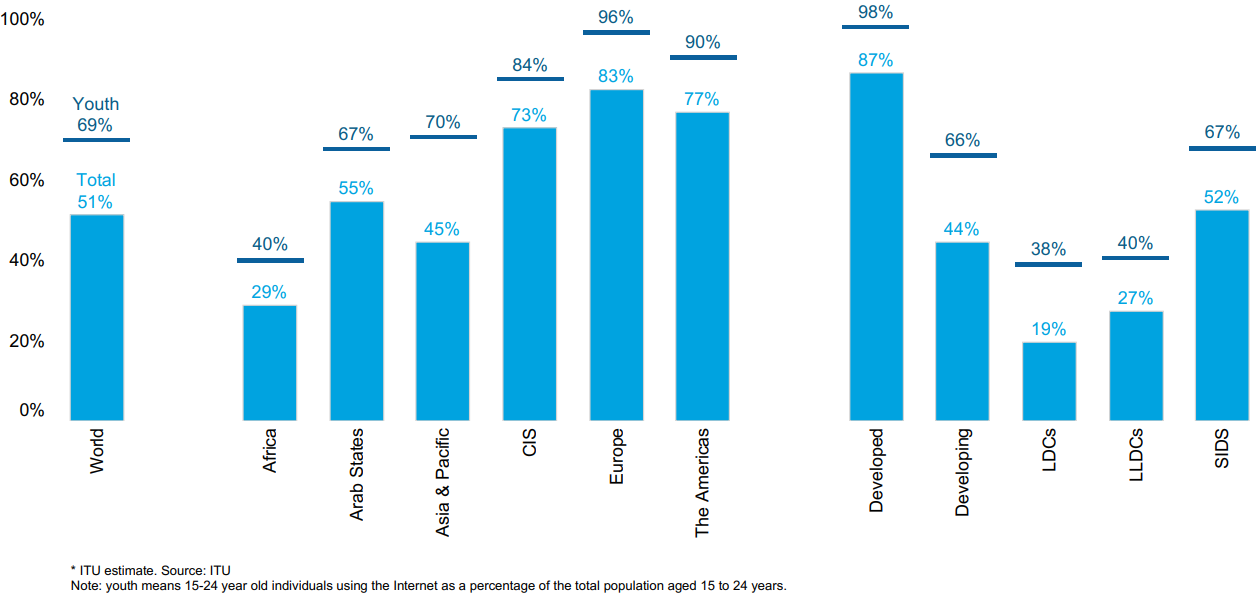
\includegraphics[width=1\textwidth]{images/itu-individuals-using-internet.png}}
\caption*{Fonte: \citeonline{Itu2020}}
\end{figure}

Vale ressaltar que as TICs não se limitam a soluções baseadas em Internet, muitas delas, inclusive, têm a capacidade de funcionar totalmente \textit{offline}. Com isso, em cenários onde o acesso à rede ainda é escasso (como em zonas rurais), também é possível promover o uso das TICs. Nesse sentido, de acordo com o último relatório do \citeonline{Itu2020}, em apenas 8 das 73 economias analisadas menos da metade da população possui \textit{smartphones} (\autoref{fig:itu-donos-smartphones}). No Brasil, por exemplo, estima-se que 80-89\% das pessoas possui ao menos um dispositivo.

\begin{figure}[htbp]
\caption{ITU: Porcentagem de indivíduos que possuem ao menos um \textit{smartphone}.}
\label{fig:itu-donos-smartphones}
\centerline{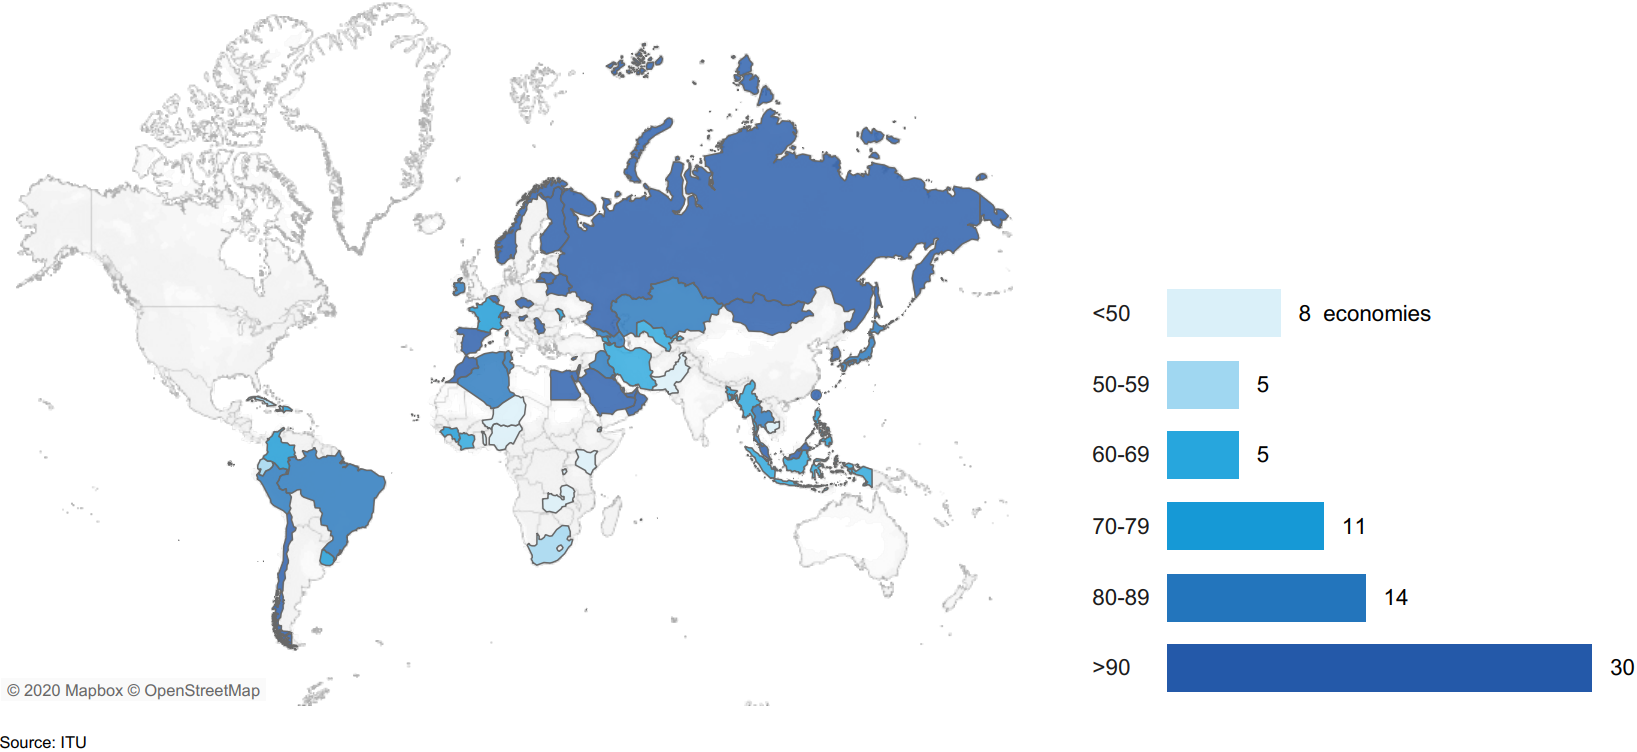
\includegraphics[width=1\textwidth]{images/itu-individuals-owning-mobile-phone.png}}
\caption*{Fonte: \citeonline{Itu2020}}
\end{figure}

Sendo assim, é possível inferir que o desenvolvimento de aplicativos móveis seria uma abordagem efetiva no Brasil. Além disso, é sabido que o público jovem é mais ativo no uso da Internet \cite{Itu2020}, o que pode servir de insumo para requisitos e especificações técnicas de soluções. Portanto, tais fatos podem direcionar de forma assertiva o desenvolvimento de aplicações adequadas ao contexto de seus usuários, especialmente no domínio educacional.%, visando o suporte às línguas oral e de sinais, por exemplo.

\subsection{Abordagens Pedagógicas}
\label{fundamentacao-teorica:tic:educacao}

\citeonline{Cilli2017} relatam que a educação contou com vários tipos de abordagens nos últimos anos, as quais se mesclavam em alguns momentos e se distanciavam em outros, mas em cada uma delas foram utilizadas as tecnologias disponíveis de acordo com a forma pela qual se acreditava que ocorria o processo de ensino-aprendizagem.

No Brasil, a partir dos estudos de \citeonline{Mizukami1986}, as abordagens Tradicional, Comportamentalista, Humanista, Sociocultural e Cognitivista foram idealizadas, tendo em vista as práticas educacionais nacionais. De forma complementar, as teorias da Aprendizagem Significativa \cite{Ausubel1980} e Inteligências Múltiplas \cite{Gardner1995} também representam abordagens pedagógicas importantes no processo de ensino moderno. Nesse contexto, \citeonline{Cilli2017} sintetizam essas abordagens conceitualmente:

\begin{itemize}
    \item \textbf{Tradicional}: Trata-se de uma concepção e uma prática educacional que persiste no tempo, em suas diferentes formas, na qual o adulto é considerado como um homem acabado, ``pronto'' e o aluno como um ``adulto em miniatura'', que precisa ser atualizado \cite{Cilli2017, Mizukami1986};
    \item \textbf{Comportamentalista}: Nessa abordagem o conhecimento é considerado uma nova descoberta para o aluno. Contudo, considera-se que esse novo conhecimento já se encontra presente na realidade exterior do aluno. Em outras palavras, o ser humano é uma consequência das influências ou forças existentes no meio ambiente e, dessa forma, surge a hipótese de que o homem não é um ser livre, pois depende do conhecimento que já existe fora dele para sobreviver. Portanto, o conhecimento é o resultado direto da experiência, e o comportamento humano deve ser estruturado indutivamente, via experiência \cite{Cilli2017, Mizukami1986};
    \item \textbf{Humanista}: Essa abordagem enfatiza o papel do sujeito como principal elaborador do conhecimento humano. Propõe que o crescimento deve ser centrado no desenvolvimento da personalidade do indivíduo, na sua capacidade de atuar como uma pessoa integrada, uma vez que o homem é considerado como uma pessoa situada no mundo. Não existem modelos prontos nem regras a seguir, mas um processo de vir a ser. O objetivo do ser humano é a auto realização ou uso pleno de suas potencialidades e capacidades \cite{Cilli2017, Mizukami1986};
    \item \textbf{Sociocultural}: A partir das obras de Paulo Freire, enfatiza-se os aspectos sócio-político-culturais, havendo uma grande preocupação com a cultura popular. Cabe enfatizar que essa preocupação ocorre desde a II Guerra Mundial com um aumento crescente até nossos dias, uma vez que o homem está inserido no contexto histórico, o que indica que a ação educativa deve promover o indivíduo como sendo único dentro da sociedade a qual pertence \cite{Cilli2017, Mizukami1986};
    \item \textbf{Cognitivista}: Organização do conhecimento a qual ocorre por meio do processamento de informações, dos estilos de pensamento ou estilos cognitivos e dos comportamentos relativos à tomada de decisões, dentre outros. Nesse sentido, o homem e mundo são analisados conjuntamente, já que o conhecimento é o produto da interação entre eles \cite{Cilli2017, Mizukami1986};
    \item \textbf{Teoria da Aprendizagem Significativa}: Processo pelo qual uma nova informação se relaciona de maneira não arbitrária e substantiva na estrutura cognitiva do aluno. Em outras palavras, ela não ocorre de forma literal, não é armazenada na memória da mesma forma que o aluno ouviu ou leu a informação \cite{Cilli2017, Ausubel1980};
    \item \textbf{Teoria das Inteligências Múltiplas}: Desenvolvida por Howard Gardner no início da década de 1980, na Universidade de Harvard, onde o autor é professor. Por meio dessa teoria foi possível identificar, de forma clara e objetiva, as necessidades atuais dos alunos em suas várias faixas etárias. Por isso, essa teoria é utilizada como embasamento na prática pedagógica de inúmeras escolas no mundo inteiro. De acordo com Gardner todos nós possuímos, pelo menos, nove tipos diferentes de inteligência, chamadas por ele de Inteligências Múltiplas. É importante observar que Inteligência diz respeito à forma como as pessoas resolvem problemas e interagem com a sociedade com a qual convivem \cite{Cilli2017, Gardner1995}:
    \subitem 1. \textit{Linguística ou verbal}: domínio e gosto pelos idiomas e pelas palavras.  Ex: poetas, escritores e linguistas;
    \subitem 2. \textit{Lógico matemática}:  capacidade de confrontar e avaliar objetos e abstrações. Facilidade para o raciocínio dedutivo e para solucionar problemas matemáticos. Ex: engenheiros, matemáticos, físicos;
    \subitem 3. \textit{Musical}: facilidade em reproduzir padrões musicais de ouvido além de discernir os diferentes timbres e ritmos. Ex: músicos, intérpretes, compositores;
    \subitem 4. \textit{Visuespacial}: capacidade de compreender o mundo visual com precisão e reproduzi-los mentalmente mesmo sem estímulos físicos. Ex: arquitetos, escultores, cartógrafos, jogadores de xadrez;
    \subitem 5. \textit{Corporal cinestésica}: capacidade de controlar e orquestrar movimentos do corpo. Ex: atores, esportistas, dançarinos;
    \subitem 6. \textit{Intrapessoal}: capacidade de se conhecer. Ex: psicólogos, psicanalistas, neurologistas e conselheiro;
    \subitem 7. \textit{Interpessoal}: habilidade de entender as interações, motivações e desejos dos outros. Ex: políticos, religiosos, professores;
    \subitem 8. \textit{Naturalista}: sensibilidade para compreender e organizar os objetos, fenômenos e padrões da natureza, como reconhecer plantas, animais e minerais. Ex: geólogos, biólogos;
    \subitem 9. \textit{Existencial}: capacidade de refletir e ponderar sobre questões fundamentais da existência. Ex: Jean-Paul Sartre, Papa Francisco, Dalai Lama. 
\end{itemize}

Tendo em vista as abordagens em questão, \citeonline{Cilli2017} detalha cada um delas no contexto do uso da tecnologia como ferramenta de apoio ao processo de ensino e aprendizagem. Desta forma, a \autoref{tab:abordagens-pedagogicas:tecnologia} foi idealizada com o objetivo de sintetizar tais tecnologias, as quais nem sempre são citadas diretamente, pois o conceito de tecnologia pode ser relativizado dependendo da abordagem.

\begin{table}[htbp]
\caption{Tecnologias/Recursos das abordagens pedagógicas}
\label{tab:abordagens-pedagogicas:tecnologia}
\begin{tabularx}{\textwidth}{p{3.5cm}|X} \hline
\textbf{Abordagem} & \textbf{Recursos/Tecnologias} \\ \hline
Tradicional & As tecnologias mais utilizadas são aquelas que permitem maior intensidade na concentração do aluno para que este possa memorizar a maior quantidade de informações possível. Por isso, os recursos de ensino mais utilizados são: \textbf{livro, caderno, lousa, e as ações do professor enquanto transmissor de informações}. \\ \hline
Comportamentalista & Recursos que permitem o uso de estimulo e resposta como o estudo dirigido e a instrução programada, cujos \textbf{materiais já trazem as respostas dos exercícios e tentam prever possíveis questionamentos que os alunos possam fazer a respeito do que estão aprendendo}, com base no comportamento dos mesmos. \\ \hline
Humanista & Qualquer tipo de recurso que facilite tanto o desenvolvimento racional como o emocional, e os brinquedos pedagógicos tem especial destaque nesse processo por serem capazes de simular situações de convívio com a família e com a sociedade em geral, permitindo assim com que o aluno se expresse e reconheça a importância da forma como essas expressões ocorrem, principalmente no que diz respeito a seu desenvolvimento emocional. Aqui estão presentes recursos como \textbf{fantoches, roupas para teatro, livros interativos, histórias contadas via meios digitais}. \\ \hline
Sociocultural & Recursos com os quais os alunos convivem no seu dia a dia, também podem ser considerados como recursos tecnológicos para a aprendizagem. Aqui podemos citar a \textbf{televisão, vídeos, imagens de realidades a serem entendidas}. \\ \hline
Cognitivista & Recursos tecnológicos como \textbf{computadores, tablets e \textit{smartphones}} permitem com que os alunos participem de jogos digitais, pesquisas na Internet e construção de textos de forma colaborativa. \\ \hline
Teoria da Aprendizagem Significativa & Esta teoria nos inspira a refletir sobre a estrutura em que os diversos \textbf{conteúdos são desenvolvidos para que posteriormente sejam disponibilizados em recursos tecnológicos}, ou, então, de que forma o professor planejará as atividades para que todo o processo seja organizado de forma significativa e atenda aos objetivos propostos. \\ \hline
Teoria das Inteligências Múltiplas & Assim como a Teoria da Aprendizagem Significativa, nos estimula a analisar que tipo de conteúdo está sendo veiculado para a promoção do ensino e da aprendizagem. Contudo, no caso da Teoria das Inteligências Múltiplas, também podemos observar a qualidade das atividades que são propostas para garantir que os principais tipos de competências e habilidades realmente sejam contemplados no processo. \\ \hline
\end{tabularx}
\caption*{Fonte: \citeonline{Cilli2017}.}
\end{table}

Com isso, foi possível obter uma visão geral das principais abordagens pedagógicas existentes. Entretanto, elas devem se adaptar em muitos aspectos, visando a educação inclusiva, como visto anteriormente. Nesse sentido, para que a tecnologia possa apoiar tais abordagens em um contexto inclusivo, a tecnologia assistiva é fundamental, pois potencializa o aprendizado de PcD. A seção a seguir trata desse tema em detalhes.

\subsection{Tecnologia Assistiva}
\label{fundamentacao-teorica:tic:assistiva}

Segundo \citeonline{Bersch2017}, a Tecnologia Assistiva (TA) é um termo que identifica o conjunto de recursos e serviços que contribuem para proporcionar ou ampliar habilidades funcionais de PcD e consequentemente promover independência e inclusão. Já \citeonline{Cook2015} a definem como uma ampla gama de equipamentos, serviços, estratégias e práticas concebidas e aplicadas para reduzir os problemas encontrados pelas PcD.

No Brasil, em 2006, foi instituído o Comitê de Ajudas Técnicas (CAT), estabelecido pelo Decreto nº 5.296/2004 no âmbito da Secretaria Especial dos Direitos Humanos da Presidência da República, com o objetivo de aperfeiçoar, dar transparência e legitimidade ao desenvolvimento da TA. No início, ``Ajudas Técnicas'' era um termo utilizado, mas atualmente foi descontinuado em detrimento da TA \cite{Cat2008}. De forma adicional, \citeonline{Cat2008} define a TA como:

\begin{citacao}
Uma área do conhecimento, de característica interdisciplinar, que engloba produtos, recursos, metodologias, estratégias, práticas e serviços que objetivam promover a funcionalidade, relacionada à atividade e participação, de PcD, incapacidades ou mobilidade reduzida, visando sua autonomia, independência, qualidade de vida e inclusão social \cite{Cat2008}.
\end{citacao}

\citeonline{Bersch2017}, por sua vez, vem contribuindo consistentemente na área da TA. Nesse sentido, a autora propõem a classificação do conceito de TA em algumas categorias. No contexto deste trabalho, a categoria destinada a \aspas{auxílios para melhorar a função auditiva e recursos utilizados para traduzir os conteúdos de áudio em imagens, texto e língua de sinais} merece destaque, pois envolve desde aparelhos para surdez até o uso de dispositivos móveis como soluções de TA.%as quais estão listadas a seguir, com destaque para a categoria destinada às recursos/serviços para surdos:

%\begin{itemize}
%\item Auxílios para a vida diária e vida prática;%:  Materiais e produtos para auxílio em tarefas rotineiras tais como comer, cozinhar, vestir-se, tomar banho e executar necessidades pessoais, manutenção da casa etc.
%\item Comunicação Aumentativa e Alternativa (CAA);%:  Recursos, eletrônicos ou não, que permitem a comunicação expressiva e receptiva das pessoas sem a fala ou com limitações da mesma. Recursos como as pranchas de comunicação, construídas com simbologia gráfica (BLISS, PCS e outros), letras ou palavras escritas, são utilizados pelo usuário da CAA para expressar;
%\item Recursos de acessibilidade ao computador;%:  Equipamentos de entrada e saída (síntese de voz, Braille), auxílios alternativos de acesso (ponteiras de cabeça, de luz), teclados modificados ou alternativos, acionadores, softwares especiais (de reconhecimento de voz, etc.), que permitem as pessoas com deficiência a usarem o computador.
%\item Sistemas de controle de ambiente;%:  Sistemas eletrônicos que permitem as pessoas com limitações moto-locomotoras, controlar remotamente aparelhos eletro-eletrônicos, sistemas de segurança, entre outros, localizados em seu quarto, sala, escritório, casa e arredores.
%\item Projetos arquitetônicos para acessibilidade;%:  Adaptações estruturais e reformas na casa e/ou ambiente de trabalho, através de rampas, elevadores, adaptações em banheiros entre outras, que retiram ou reduzem as barreiras físicas, facilitando a locomoção da pessoa com deficiência.
%\item Órteses e próteses;%:  Troca ou ajuste de partes do corpo, faltantes ou de funcionamento comprometido, por membros artificiais ou outros recurso ortopédicos (talas, apoios etc.). Inclui-se os protéticos para auxiliar nos deficits ou limitações cognitivas, como os gravadores de fita magnética ou digital que funcionam como lembretes instantâneos.
%\item Adequação postural;%:  Adaptações para cadeira de rodas ou outro sistema de sentar visando o conforto e distribuição adequada da pressão na superfície da pele (almofadas especiais, assentos e encostos anatômicos), bem como posicionadores e contentores que propiciam maior estabilidade e postura adequada do corpo através do suporte e posicionamento de tronco/cabeça/membros.
%\item Auxílios de mobilidade;%:  Cadeiras de rodas manuais e motorizadas, bases móveis, andadores, scooters de 3 rodas e qualquer outro veículo utilizado na melhoria da mobilidade pessoal.
%\item Auxílios para ampliação da função visual e recursos que traduzem conteúdos visuais em áudio ou informação tátil;%:  Auxílios para grupos específicos que inclui lupas e lentes, Braille para equipamentos com síntese de voz, grandes telas de impressão, sistema de TV com aumento para leitura de documentos, publicações etc.
%\item \textbf{Auxílios para melhorar a função auditiva e recursos utilizados para traduzir os conteúdos de áudio em imagens, texto e língua de sinais.};%:  Auxílios que inclui vários equipamentos (infravermelho, FM), aparelhos para surdez, telefones com teclado — teletipo (TTY), sistemas com alerta táctil-visual, entre outros.
%\item Mobilidade em veículos;%:  Acessórios e adaptações que possibilitam a condução do veículo, elevadores para cadeiras de rodas, camionetas modificadas e outros veículos automotores usados no transporte pessoal.
%\item Esporte e Lazer.
%\end{itemize}

Nesse cenário, é evidente que as TICs estão implicitamente relacionadas aos recursos de TA, pois são a base para muitas dessas soluções. Sendo assim, é possível inferir que essas tecnologias, quando aplicadas em um contexto de inclusão, podem derivar ferramentas poderosas de TA. Portanto, domínios complexos, como o da educação inclusiva, podem se beneficiar da ubiquidade das TICs e criar ambientes de ensino mais dinâmicos e adequados às necessidades de seus aprendizes.

Em especial, considerando a educação inclusiva para surdos, as TA são ferramentas importantes para que eles tenham alternativas em termos de acessibilidade e, idealmente, sejam incluídos em todos os sentidos. De acordo com \citeonline{Bersch2017}, no campo educacional, pode haver uma distinção sutil entre TA e tecnologia educacional. Para não haver dúvidas, a autora sugere que se façam três perguntas:

\begin{enumerate}
\item \aspas{O recurso está sendo utilizado por um aluno que enfrenta alguma barreira em função de sua deficiência (sensorial, motora ou intelectual) e este recurso/estratégia o auxilia na superação desta barreira?} \cite{Bersch2017};
\item \aspas{O recurso está apoiando o aluno na realização de uma tarefa e proporcionando a ele a participação autônoma no desafio educacional, visando sempre chegar ao objetivo educacional proposto?} \cite{Bersch2017};
\item \aspas{Sem este recurso o aluno estaria em desvantagem ou excluído de participação?} \cite{Bersch2017}.
\end{enumerate}

Tendo respostas afirmativas para as três questões, \citeonline{Bersch2017} afirma que o recurso pode ser classificado como TA, mesmo quando ele se denomina como tecnologia educacional. Isso porque, de modo geral, toda a TA é uma tecnologia educacional, desde que esteja no domínio da educação. Com isso, é possível identificar de forma simples soluções/ferramentas sob a perspectiva teórica correta.

Nesta seção foi possível entender o conceito de TA e sua relação intrínseca com a educação inclusiva, pois a TA pode prover soluções robustas o suficiente para que sinalizantes e ouvintes possam interagir de forma mais legítima/inclusiva. %Com isso, a seguir, discutimos um pouco sobre a perspectiva de desenvolvimento desta proposta, juntamente com seus desafios e eventuais problemas.

\subsection{Desafios e Problemas}
\label{fundamentacao-teorica:tic:desafios}

Um dos maiores desafios das TICs é atingir a onipresença em nível global, pois em países desenvolvidos essa etapa já está praticamente concluída, tendo em vista alguns parâmetros relevantes como o acesso à Internet e o uso de \textit{smartphones}. Particularmente, países em desenvolvimento também apresentam um crescimento consistente no uso dessas tecnologias, sobretudo tendo em vista o público jovem \cite{Itu2020}. Esse cenário, aliado à necessidade de democratizar a educação inclusiva/bilíngue para surdos, sugere uma linha de pesquisa interessante.

De forma complementar, as práticas pedagógicas também devem ser levadas em conta, pois fazem parte do processo ensino-aprendizagem e, consequentemente, influenciarão a dinâmica social e cultural dos alunos. Por isso, propor soluções tecnológicas que sejam adaptáveis a diferentes contextos educacionais é um desafio evidente. Para isso, investigar formas de aumentar a sinergia entre educação inclusiva e TA pode contribuir significativamente nessa perspectiva.

Outro desafio relevante diz respeito aos padrões de desenvolvimento das soluções educacionais em questão. Nesse sentido, o uso de boas práticas que favoreçam o compartilhamento de recursos e informações é essencial. Para isso, técnicas de reúso da Engenharia de Software (ES) podem ser efetivas. Adicionalmente, iniciativas de educação aberta vêm ganhando força e introduziram o conceito de Recursos Educacionais Abertos (REAs), os quais promovem soluções de ensino e aprendizagem públicas, que podem representar um meio para a disseminação da educação inclusiva.

Sendo assim, é possível concluir que, para a criação de ambientes educacionais mais inclusivos, é necessário levar em consideração uma série de aspectos. Primeiramente, tratar as línguas de sinais com a mesma importância da língua falada, favorecendo a diversidade e a disseminação da cultura surda. Nesse contexto, o uso de TICs é importante para que as práticas pedagógicas sejam devidamente apoiadas por meio de recursos educacionais efetivos, os quais, muitas vezes, se caracterizam como TA. Por fim, identificar o estado da prática, considerando o ensino e aprendizagem com línguas de sinais mediante o uso das TICs, tornou-se uma premissa importante para a continuidade deste trabalho. Assim, um estudo sistemático foi conduzido, o qual é descrito em detalhes no \autoref{chapter:mapeamento-sistematico}.

\section{Considerações Finais}
\label{fundamentacao-teorica:fim}

Ao fim desta seção foi possível obter uma visão geral sobre os temas que fundamentam este trabalho. De modo geral, as línguas de sinais foram apresentadas, com ênfase na Libras e nas boas práticas da educação inclusiva identificadas na literatura. Além disso, é importante observar que a Libras, assim como qualquer outra língua, possui completude linguística e variações regionais/culturais, o que deve ser levado em conta para a inclusão efetiva dos surdos no contexto escolar, preferencialmente por meio da educação bilíngue (Libras/Português).

Em outra perspectiva, as TICs podem ser grandes aliadas para a desmistificação do processo de inclusão dos surdos. Isso porque essas tecnologias nunca estiveram tão presentes no nosso cotidiano, o que permite a reflexão sobre potenciais soluções de TA no contexto educacional, visando a sinergia e inclusão entre alunos sinalizantes e ouvintes.

Entretanto, essas são percepções iniciais, fundamentadas apenas com base nos conceitos apresentados nesta seção. Sendo assim, a seguir apresenta-se a condução de um Mapeamento Sistemático da Literatura, cujo objetivo é identificar o estado da prática com relação aos conceitos de: (i) línguas de sinais; (ii) ensino e aprendizagem; e (iii) tecnologias. %Com isso, a presente discussão será formalmente delineada considerando questões de pesquisa cuidadosamente definidas para esta proposta.
